    
\section{实验步骤}

\begin{enumerate}
    \item 打开 JLT-1 理论力学多功能实验台电源,在实验台控制面板上以用户名 01、密码 01 登陆。 
    \item 选择“摩擦因数测量”实验选项,进入实验界面。
    \item 检查摩擦系数测定装置和材料。滑块底板两种材质:铝合金、有机玻璃;平板两种材质:不锈钢、铝合金(任选一种进行实验)。实验要求测量两种滑块在不锈钢或者铝合金上的摩擦系数。
    \item 静滑动摩擦系数测量:
        \begin{enumerate}
            \item 预先设置较大的平板坡度,使滑块可以从平板上方顺利滑下(注意,滑块均应轻轻放置于平板上,勿重压);
            \item 摇动升降手柄,间隔 1$^\circ$ 以上逐步降低平板倾斜角 $\varphi$,直至滑块轻置于平板上后不再发生滑动;
            \item 以坡度测量仪测量此时的平板倾斜角 $\varphi_s$,并记录。注意:每一倾角下检测三次是否滑动,三次选择不同的放置地点(建议为平板最顶部、光电管 L1 处和光电管 L2 处)。
            \item 改变滑块材质,重复以上实验。
        \end{enumerate}
    \item 动滑动摩擦系数测量:
        \begin{enumerate}
            \item 用游标卡尺测量滑块两挡板间距离 $s_1$,并记录;
            \item 设置平板倾斜角大于最大静摩擦角,避开“黏滑现象”,确保滑块可顺畅滑下。用坡度测量仪测量并记录此时倾斜角 $\varphi$,并在平台触控面板输入角度值;
            \item 在触控面板点击“开始”,将滑块轻放于平板顶部并释放,使其自主滑下。待滑块通过两光电管后,触控面板显示实验数据。每组材质和坡度角下重复测量 4~6 次;
            \item 记录 $t_1$~$t_3$ 三个原始时间数据;
            \item 改变平板倾斜角,重复步骤 1~4,测试两个不同倾斜角(间隔 5° 以上);
            \item 更换滑块材质,重复上述实验。
        \end{enumerate}
    \item 实验完毕,将实验器材恢复至原位,关闭实验台电源,并打扫清理实验工位。
\end{enumerate}

\section{实验数据处理}
\subsection{静滑动摩擦系数测量一}
滑块材质:有机玻璃

平板材质:铝
\subsubsection{实验原始数据}

\begin{table}[h!]
    \centering
    \renewcommand{\arraystretch}{1.5}
    \setlength{\tabcolsep}{8pt}
    \begin{tabular}{|c|c|c|c|c|c|}
    \hline
    \textbf{No.} & \textbf{倾斜角/°} & 测试 1 & 测试 2 & 测试 3 \\ \hline
    1 & 19.2° & 0 & 0 & 0 \\ \hline
    2 & 19.6° & 0 & 0 & 0 \\ \hline
    3 & 20.9° & 0-1 & 0 & 0 \\ \hline
    4 & 21.5° & 0 & 0 & 0 \\ \hline
    5 & 22.1° & 0-1 & 0-1 & 0 \\ \hline
    6 & 22.5° & 0-1 & 0-1 & 0-1\\ \hline
    7 & 22.7° & 1 & 1 & 0-1 \\ \hline
    8 & 23.4° & 1 & 1 & 1 \\ \hline
    9 & 24.1° & 1 & 1 & 1 \\ \hline
    10 & 24.7° & 1 &1 & 1 \\ \hline
    \end{tabular}
    \caption{铝 - 玻璃静滑动摩擦系数测量数据}
    \label{tab:static_friction_data}
\end{table}
备注:静止记为 0,滑动记为 1,0-1 代表有时滑动,有时静止。
\subsubsection{静滑动摩擦系数计算}
静滑动摩擦系数为:
$$  
f_{s.1}=\tan \varphi_{s.1}=\tan 21.5°=0.3939
$$ 
$$ 
f_{s.3}=\tan \varphi_{s.1}=\tan 22.1°=0.4061
$$
\subsection{静滑动摩擦系数测量二}
滑块材质:铝

平板材质:铝
\subsubsection{实验原始数据}

\begin{table}[h!]
    \centering
    \renewcommand{\arraystretch}{1.5}
    \setlength{\tabcolsep}{8pt}
    \begin{tabular}{|c|c|c|c|c|c|}
    \hline
    \textbf{No.} & \textbf{倾斜角/°} & 测试 1 & 测试 2 & 测试 3 \\ \hline
    1 & 14.5° & 0 & 0 & 0 \\ \hline
    2 & 15.4° & 0 & 0 & 0 \\ \hline
    3 & 17.1° & 0 & 0 & 0 \\ \hline
    4 & 17.6° & 0 & 0-1 & 0 \\ \hline
    5 & 18.7° & 0-1 & 0-1 & 0-1 \\ \hline
    6 & 19.0° & 0-1 & 0 & 0-1\\ \hline
    7 & 19.6° & 1 & 1 & 1 \\ \hline
    8 & 21.3° & 1 & 1 & 1 \\ \hline
    9 & 22.9° & 1 & 1 & 1 \\ \hline
    10 & 23.8° & 1 &1 & 1 \\ \hline
    \end{tabular}
    \caption{铝 - 铝静滑动摩擦系数测量数据}
    \label{tab:static_friction_data}
\end{table}

\subsubsection{静滑动摩擦系数计算}
静滑动摩擦系数为:
$$  
f_{s.1}=\tan \varphi_{s.1}=\tan 17.6°=0.3172
$$ 
$$ 
f_{s.3}=\tan \varphi_{s.1}=\tan 19.0°=0.3443
$$
% \subsection{动滑动摩擦系数测量一}

% 滑块材质:有机玻璃
% 平板材质:铝
% 滑块挡板间距离$s_1= 30mm$
% \subsubsection{实验原始数据}
% \begin{table}[h!]
%     \centering
%     \renewcommand{\arraystretch}{1.5}
%     \setlength{\tabcolsep}{8pt}
%     \begin{tabular}{|c|c|c|c|c|c|}
%     \hline
%     \textbf{No.} & \textbf{倾斜角/°} & 测试 1 & 测试 2 & 测试 3 \\ \hline
%     1 & 14.5° & 0 & 0 & 0 \\ \hline
%     2 & 15.4° & 0 & 0 & 0 \\ \hline
%     3 & 17.1° & 0 & 0 & 0 \\ \hline
%     4 & 17.6° & 0 & 0-1 & 0 \\ \hline
%     5 & 18.7° & 0-1 & 0-1 & 0-1 \\ \hline
%     6 & 19.0° & 0-1 & 0 & 0-1\\ \hline
%     7 & 19.6° & 1 & 1 & 1 \\ \hline
%     8 & 21.3° & 1 & 1 & 1 \\ \hline
%     9 & 22.9° & 1 & 1 & 1 \\ \hline
%     10 & 23.8° & 1 &1 & 1 \\ \hline
%     \end{tabular}
%     \caption{铝 - 铝静滑动摩擦系数测量数据}
%     \label{tab:lvlvstatic_friction_data}
% \end{table}


\subsection{动滑动摩擦系数测量一}

滑块材质:有机玻璃
平板材质:铝
滑块挡板间距离 $s_1=30.0\,\mathrm{mm}=0.0300\,\mathrm{m}$
其中 $\varphi=25.7^\circ$,$g=9.80\,\mathrm{m/s^2}$。

\subsubsection{实验原始数据}
\begin{table}[h!]
    \centering
    \renewcommand{\arraystretch}{1.5}
    \setlength{\tabcolsep}{8pt}
    \begin{tabular}{|c|c|c|c|c|c|}
    \hline
    \textbf{No.} & $t_1$/ms & $t_2$/ms & $t_3$/ms & $t_4$/ms & $f_d$ \\ \hline
    1 & 80 & 61 & 643 & 633.5 & 0.404 \\ \hline
    2 & 83 & 65 & 665 & 656.0 & 0.408 \\ \hline
    3 & 93 & 73 & 775 & 765.0 & 0.412 \\ \hline
    4 & 94 & 74 & 776 & 766.0 & 0.412 \\ \hline
    5 & 88 & 64 & 685 & 673.0 & 0.403 \\ \hline
    6 & 106 & 87 & 852 & 842.5 & 0.416 \\ \hline
    7 & 98 & 78 & 776 & 766.0 & 0.413 \\ \hline
    8 & 101 & 101 & 847 & 847.0 & 0.424 \\ \hline
    \end{tabular}
    \caption{铝 - 有机玻璃动滑动摩擦系数测量数据 (一)}
    \label{tab:dynamic_friction_data}
\end{table}

剔除偏差过大的数据后,平均动摩擦系数为:
$$
\overline{f_d} = 0.412
$$

\subsection{动滑动摩擦系数测量二}

滑块材质:有机玻璃

平板材质:铝

滑块挡板间距离 $s_1=30.0\,\mathrm{mm}=0.0300\,\mathrm{m}$

其中 $\varphi=27.5^\circ$,$g=9.80\,\mathrm{m/s^2}$。

\subsubsection{实验原始数据}
\begin{table}[h!]
    \centering
    \renewcommand{\arraystretch}{1.5}
    \setlength{\tabcolsep}{8pt}
    \begin{tabular}{|c|c|c|c|c|c|}
    \hline
    \textbf{No.} & $t_1$/ms & $t_2$/ms & $t_3$/ms & $t_4$/ms & $f_d$ \\ \hline
    1 & 69 & 47 & 544 & 533.0 & 0.382 \\ \hline
    2 & 59 & 41 & 482 & 473.0 & 0.372 \\ \hline
    3 & 69 & 51 & 562 & 553.0 & 0.394 \\ \hline
    4 & 65 & 50 & 515 & 507.5 & 0.394 \\ \hline
    5 & 74 & 52 & 567 & 556.0 & 0.390 \\ \hline
    6 & 72 & 51 & 544 & 533.5 & 0.389 \\ \hline
    7 & 69 & 51 & 544 & 535.0 & 0.393 \\ \hline
    8 & 79 & 56 & 591 & 579.5 & 0.395 \\ \hline
    \end{tabular}
    \caption{铝 - 有机玻璃动滑动摩擦系数测量数据(二)}
    \label{tab:dynamic_friction_data2}
\end{table}

剔除偏差过大的数据后,平均动摩擦系数为:
$$
\overline{f_d} =0.389
$$

\subsection{动滑动摩擦系数测量二}

滑块材质:铝

平板材质:铝

滑块挡板间距离 $s_1=30.0\,\mathrm{mm}=0.0300\,\mathrm{m}$

其中 $\varphi=23.0^\circ$,$g=9.80\,\mathrm{m/s^2}$。

\subsubsection{实验原始数据}
\begin{table}[h!]
    \centering
    \renewcommand{\arraystretch}{1.5}
    \setlength{\tabcolsep}{8pt}
    \begin{tabular}{|c|c|c|c|c|c|}
    \hline
    \textbf{No.} & $t_1$/ms & $t_2$/ms & $t_3$/ms & $t_4$/ms & $f_d$ \\ \hline
    1 & 60  & 28  & 377 & 361 & 0.249 \\ \hline
    2 & 50  & 27  & 349 & 337.5 & 0.257 \\ \hline
    3 & 46  & 28  & 334 & 325 & 0.281 \\ \hline
    4 & 59  & 33  & 382 & 369 & 0.304 \\ \hline
    5 & 50  & 28  & 354 & 343 & 0.272 \\ \hline
    6 & 55  & 32  & 396 & 384.5 & 0.311 \\ \hline
    7 & 51  & 33  & 401 & 392 & 0.334 \\ \hline
    8 & 51  & 28  & 354 & 342.5 & 0.268 \\ \hline
    \end{tabular}
    \caption{铝 - 铝动滑动摩擦系数测量数据(一)}
    \label{tab:dynamic_friction_data2}
\end{table}

剔除偏差过大的数据后,平均动摩擦系数为:
$$
\overline{f_d} = 0.28
$$

\subsection{动滑动摩擦系数测量二}

滑块材质:铝

平板材质:铝

滑块挡板间距离 $s_1=30.0\,\mathrm{mm}=0.0300\,\mathrm{m}$


其中 $\varphi=24.2^\circ$,$g=9.80\,\mathrm{m/s^2}$。

\subsubsection{实验原始数据}
\begin{table}[h!]
    \centering
    \renewcommand{\arraystretch}{1.5}
    \setlength{\tabcolsep}{8pt}
    \begin{tabular}{|c|c|c|c|c|c|}
    \hline
    \textbf{No.} & $t_1$/ms & $t_2$/ms & $t_3$/ms & $t_4$/ms & $f_d$ \\ \hline
    1 & 60 & 51 & 469 & 464.5 & 0.403 \\ \hline
    2 & 69 & 56 & 539 & 532.5 & 0.403 \\ \hline
    3 & 50 & 46 & 422 & 420.0 & 0.411 \\ \hline
    4 & 73 & 55 & 543 & 534.0 & 0.397 \\ \hline
    5 & 64 & 55 & 542 & 537.5 & 0.409 \\ \hline
    6 & 69 & 51 & 530 & 521.0 & 0.392 \\ \hline
    7 & 55 & 50 & 487 & 484.5 & 0.412 \\ \hline
    8 & 56 & 46 & 424 & 419.0 & 0.394 \\ \hline
    \end{tabular}
    \caption{铝 - 铝动滑动摩擦系数测量数据(二)}
    \label{tab:dynamic_friction_data2}
\end{table}

剔除偏差过大的数据后,平均动摩擦系数为:
$$
\overline{f_d} = 0.403
$$

\subsection{结论}
% 铝 - 玻璃静滑动摩擦系数为:
% $$  
% f_{s.1}=\tan \varphi_{s.1}=\tan 21.5°=0.3939
% $$ 
% $$ 
% f_{s.3}=\tan \varphi_{s.1}=\tan 22.1°=0.4061
% $$


% 铝 - 铝
% 静滑动摩擦系数为:
% $$  
% f_{s.1}=\tan \varphi_{s.1}=\tan 17.6°=0.3172
% $$ 
% $$ 
% f_{s.3}=\tan \varphi_{s.1}=\tan 19.0°=0.3443
% $$

% 动滑动摩擦系数
% 铝 - 有机玻璃

% $\varphi=25.7^\circ$
% $$
% \overline{f_d} = 0.412
% $$

% $\varphi=27.5^\circ$

% $$
% \overline{f_d} =0.389
% $$

% 铝 - 铝
% $\varphi=24.2^\circ$


% $$
% \overline{f_d} = 0.403
% $$

% 其中 $\varphi=23.0^\circ$

% $$
% \overline{f_d} = 0.28
% $$

\begin{table}[h!]
    \centering
    \renewcommand{\arraystretch}{1.5}
    \setlength{\tabcolsep}{10pt}
    \begin{tabular}{|c|c|c|c|c|}
    \hline
    材料组合 & 倾斜角 $\varphi$ & 静滑动摩擦系数 $f_s$ & 动滑动摩擦系数 $f_d$ \\
    \hline
    铝 - 有机玻璃 & 21.5° & 0.3939 & 0.412 ($\varphi=25.7^\circ$) \\
    铝 - 有机玻璃 & 22.1° & 0.4061 & 0.389 ($\varphi=27.5^\circ$) \\
    铝 - 铝 & 17.6° & 0.3172 & 0.28 ($\varphi=23.0^\circ$) \\
    铝 - 铝 & 19.0° & 0.3443 & 0.403 ($\varphi=24.2^\circ$) \\
    \hline
    \end{tabular}
    \caption{不同材料组合下的静、动滑动摩擦系数汇总}
    \label{tab:friction_summary}
\end{table}

\begin{figure}
    \centering
    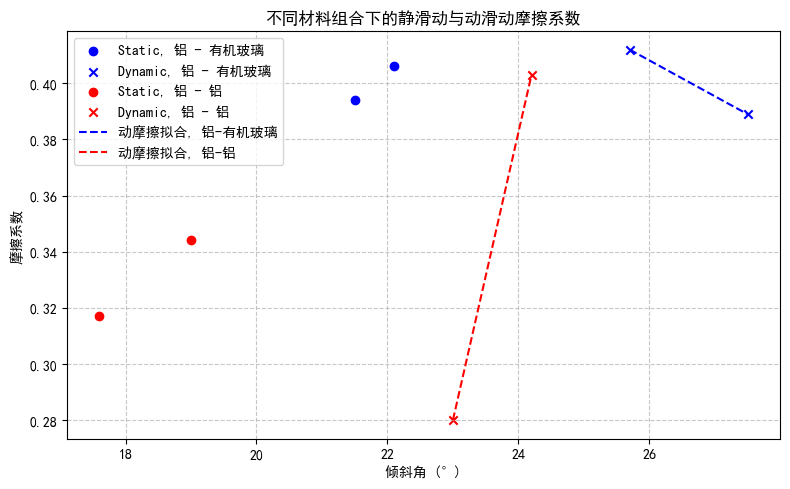
\includegraphics[width=0.8\textwidth]{image/output.png}
    \caption{摩擦系数测量实验数据}
    \label{fig:friction_experiment}
\end{figure}
\newpage
